\documentclass[border=4pt,12pt]{standalone}
% House style for redrawn exam diagrams (diagram-v4: 0.4pt lines, filled -latex arrows, fine dashes; stipple and hatching drawn as real dots/lines (no PDF/SVG patterns, so they render in every browser and at any scale); transparent background). Every figure \input's this.
\usepackage{amsmath,amssymb}
\usepackage{txfonts}
\usepackage{pdfrender,xcolor}
% \halo{text}: label on shading. The shading stops just around each letter's outline (a thin knock-out that follows the
% glyphs, like the papers' typesetting), never a box. Owner: "I don't want a box around the text".
\newcommand{\halo}[1]{\leavevmode\rlap{\pdfrender{TextRenderingMode=2,LineWidth=2.2pt,LineJoinStyle=1,StrokeColor=white,FillColor=white}#1}#1}
\usepackage{tikz,pgfplots}
\pgfplotsset{compat=1.18}
\usetikzlibrary{arrows.meta,calc,angles,quotes,patterns,patterns.meta,intersections,positioning,decorations.markings,shapes.geometric}
% Stipple and hatching are drawn as actual dots / lines clipped to the region (path picture), NOT as pattern fills:
% SVG <pattern> fills vanish or blur when browsers scale the image, so the owner could not see the shading.
% Each dot is a 0.72pt square (keeps SVGs small; reads as a dot at print size). Dots sit on one global staggered grid, so neighbouring regions line up.
\makeatletter
\newdimen\ex@x \newdimen\ex@y \newdimen\ex@xa \newdimen\ex@ya \newdimen\ex@xb \newdimen\ex@yb \newcount\ex@row
\def\exam@stipplecolor{black!75}\def\exam@dotr{0.42pt}\def\exam@dotgap{2.5}
\def\ex@rowdots{\ifdim\ex@x<\ex@xb \pgfpathrectangle{\pgfqpoint{\dimexpr\ex@x-0.36pt\relax}{\dimexpr\ex@y-0.36pt\relax}}{\pgfqpoint{0.72pt}{0.72pt}}\advance\ex@x by \exam@dotgap pt\relax\expandafter\ex@rowdots\fi}
\def\exam@stipple{%
  \pgftransformreset% dots are sized in real points even inside scaled pictures
  \pgfpointanchor{path picture bounding box}{south west}\ex@xa=\pgf@x \ex@ya=\pgf@y
  \pgfpointanchor{path picture bounding box}{north east}\ex@xb=\pgf@x \ex@yb=\pgf@y
  \pgfsetfillcolor{\exam@stipplecolor}\pgfmathsetmacro\ex@h{\exam@dotgap/2}%
  \pgfmathtruncatemacro\ex@r{floor(\ex@ya/\ex@h)-1}\ex@row=\ex@r\relax
  \ex@y=\ex@r\dimexpr\ex@h pt\relax
  \loop\ifdim\ex@y<\ex@yb
    \pgfmathtruncatemacro\ex@c{floor(\ex@xa/\exam@dotgap)-1}\ex@x=\ex@c\dimexpr\exam@dotgap pt\relax
    \ifodd\ex@row \advance\ex@x by \ex@h pt\fi
    \ex@rowdots
    \advance\ex@y by \ex@h pt \advance\ex@row by 1
    \ifnum\numexpr\ex@row-(\ex@row/4)*4\relax=0 \pgfusepath{fill}\fi% flush every 4 rows: bounded TeX memory, few clip copies in the SVG
  \repeat\pgfusepath{fill}}
\newdimen\ex@d
\def\exam@hatch#1{% #1 = 1 for /, -1 for \ ; lines 45 degrees, 3pt apart
  \pgftransformreset
  \pgfpointanchor{path picture bounding box}{south west}\ex@xa=\pgf@x \ex@ya=\pgf@y
  \pgfpointanchor{path picture bounding box}{north east}\ex@xb=\pgf@x \ex@yb=\pgf@y
  \ex@d=\dimexpr\ex@yb-\ex@ya\relax \ex@x=\dimexpr\ex@xa-\ex@d\relax
  \loop\ifdim\ex@x<\ex@xb
    \ifnum#1>0 \pgfpathmoveto{\pgfqpoint{\ex@x}{\ex@ya}}\pgfpathlineto{\pgfqpoint{\dimexpr\ex@x+\ex@d\relax}{\ex@yb}}%
    \else \pgfpathmoveto{\pgfqpoint{\ex@x}{\ex@yb}}\pgfpathlineto{\pgfqpoint{\dimexpr\ex@x+\ex@d\relax}{\ex@ya}}\fi
    \advance\ex@x by 4.24pt
  \repeat
  \pgfsetlinewidth{0.4pt}\pgfsetstrokecolor{black}\pgfusepath{stroke}}
\def\examstipple{\exam@stipple}\def\examhatch{\exam@hatch}\def\examsetstipplecolor#1{\def\exam@stipplecolor{#1}}\def\examsetdotgap#1{\def\exam@dotgap{#1}}
\makeatother
% (legacy pattern kept for old files)
% staggered stipple like the NESA papers' dotted shading
\pgfdeclarepatternformonly{exam stipple}{\pgfpointorigin}{\pgfqpoint{2.2pt}{2.2pt}}{\pgfqpoint{2.2pt}{2.2pt}}{%
  \pgfpathcircle{\pgfqpoint{0.55pt}{0.55pt}}{0.42pt}\pgfpathcircle{\pgfqpoint{1.65pt}{1.65pt}}{0.42pt}\pgfusepath{fill}}
\tikzset{
  every picture/.style={line width=0.6pt, >={Latex[length=2mm,width=1.3mm]}},
  curve/.style={line width=0.6pt},
  open arrow/.style={-{Latex[length=2mm,width=1.3mm]}},  % owner: filled -latex heads everywhere, no open chevrons
  aux/.style={dash pattern=on 2pt off 1.5pt, line width=0.6pt},
  shade/.code={\def\exA{#1}\def\exB{none}\ifx\exA\exB\else\pgfkeysalso{fill=black!18}\fi},
  shade/.default=on,
  shade dots/.style={fill=none, path picture={\examstipple}},
  stipple color/.code={\examsetstipplecolor{#1}},
  stipple gap/.code={\examsetdotgap{#1}},
  shade dense dots/.style={fill=none, stipple gap=1.6, path picture={\examstipple}},
  shade hatch/.style={fill=none, path picture={\examhatch{1}}},
  shade hatch reverse/.style={fill=none, path picture={\examhatch{-1}}},
  shade solid/.style={fill=black},
  pt/.style={circle, fill, inner sep=1.1pt},
  open pt/.style={circle, draw, fill=white, inner sep=1.1pt},
}
\pgfplotsset{
  exam axes/.style={axis lines=middle, axis line style={->}, xlabel={$x$}, ylabel={$y$},
    xlabel style={anchor=west}, ylabel style={anchor=south}, tick label style={font=\small},
    every axis plot/.append style={line width=0.6pt, black}, samples=200, clip=false,
    enlargelimits=false, axis on top},
}

\begin{document}
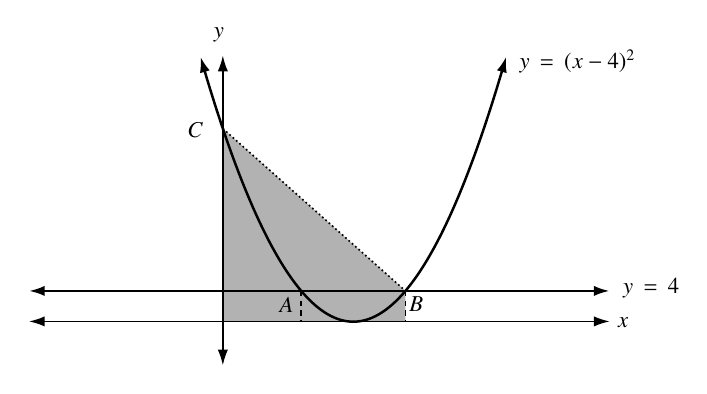
\begin{tikzpicture}[x=0.0127cm,y=-0.0127cm,every node/.style={font=\fontsize{8.2}{9.839999999999998}\selectfont}]
\fill[black!30] (210,122.1) -- (392.7,284.5) -- (392.7,315) -- (210,315) -- cycle;
\draw[<->] (16,315) -- (597,315);
\draw[<->, line width=0.9pt] (16,284.5) -- (597,284.5);
\draw[<->] (210,359) -- (210,49);
\draw[densely dotted] (210,122.1) -- (392.7,284.5);
\draw[aux] (288.4,284.5) -- (288.4,315); \draw[aux] (392.7,284.5) -- (392.7,315); \draw[aux] (210,315) -- (392.7,315);
\draw[<->, line width=0.9pt] plot[smooth] coordinates {(187.60,50.09) (191.04,61.88) (194.47,73.39) (197.91,84.64) (201.35,95.63) (204.79,106.34) (208.22,116.79) (211.66,126.97) (215.10,136.88) (218.53,146.52) (221.97,155.89) (225.41,165.00) (228.84,173.84) (232.28,182.41) (235.72,190.72) (239.16,198.75) (242.59,206.52) (246.03,214.02) (249.47,221.25) (252.90,228.22) (256.34,234.91) (259.78,241.34) (263.22,247.50) (266.65,253.39) (270.09,259.02) (273.53,264.37) (276.96,269.46) (280.40,274.28) (283.84,278.84) (287.28,283.12) (290.71,287.14) (294.15,290.89) (297.59,294.37) (301.02,297.59) (304.46,300.53) (307.90,303.21) (311.33,305.62) (314.77,307.76) (318.21,309.64) (321.65,311.24) (325.08,312.58) (328.52,313.65) (331.96,314.46) (335.39,314.99) (338.83,315.26) (342.27,315.26) (345.71,314.99) (349.14,314.45) (352.58,313.65) (356.02,312.58) (359.45,311.24) (362.89,309.63) (366.33,307.75) (369.77,305.61) (373.20,303.20) (376.64,300.52) (380.08,297.57) (383.51,294.36) (386.95,290.87) (390.39,287.12) (393.82,283.10) (397.26,278.82) (400.70,274.26) (404.14,269.44) (407.57,264.35) (411.01,258.99) (414.45,253.37) (417.88,247.47) (421.32,241.31) (424.76,234.88) (428.20,228.18) (431.63,221.22) (435.07,213.98) (438.51,206.48) (441.94,198.71) (445.38,190.68) (448.82,182.37) (452.26,173.80) (455.69,164.96) (459.13,155.85) (462.57,146.48) (466.00,136.83) (469.44,126.92) (472.88,116.74) (476.31,106.29) (479.75,95.58) (483.19,84.59) (486.63,73.34) (490.06,61.82) (493.50,50.03)};
\node[inner sep=0] at (183,124) {$C$};
\node[inner sep=0] at (273.5,299) {$A$};
\node[inner sep=0] at (403,298) {$B$};
\node[inner sep=0] at (206,28.5) {$y$};
\node[inner sep=0] at (610,316) {$x$};
\node[inner sep=0] at (638.5,282) {$y\,=\,4$};
\node[inner sep=0,anchor=west] at (506,55) {$y\,=\,(x-4)^2$};
\end{tikzpicture}
\end{document}
